% ============================================================
% MASTER BOOTCAMP HANDBOOK
% From Zero to Elite Software & AI Engineer
% By Amzat Karim
% ============================================================
\documentclass[12pt, a4paper, oneside]{book}

% ---- PACKAGES ----
\usepackage[utf8]{inputenc}
\usepackage[T1]{fontenc}
\usepackage{lmodern}
\usepackage[margin=1in]{geometry}
\usepackage{graphicx}
\usepackage{xcolor}
\usepackage{hyperref}
\usepackage{listings}
\usepackage{fancyhdr}
\usepackage{titlesec}
\usepackage{enumitem}
\usepackage{tcolorbox}
\usepackage{amsmath, amssymb}
\usepackage{booktabs}
\usepackage{longtable}
\usepackage{multicol}
\usepackage{tikz}
\usepackage{parskip}
\usepackage{microtype}
\usepackage{pifont}
\usepackage{mdframed}
\usepackage{float}
\usepackage{caption}
\usepackage{tocbibind}

% ---- COLOUR DEFINITIONS ----
\definecolor{primaryblue}{HTML}{1a73e8}
\definecolor{darkbg}{HTML}{1e1e2e}
\definecolor{codebg}{HTML}{f5f5f5}
\definecolor{codegreen}{HTML}{2e7d32}
\definecolor{codepurple}{HTML}{7b1fa2}
\definecolor{codeorange}{HTML}{e65100}
\definecolor{warnyellow}{HTML}{f9a825}
\definecolor{tipgreen}{HTML}{00c853}
\definecolor{notblue}{HTML}{2196f3}
\definecolor{cautionred}{HTML}{d32f2f}

% ---- HYPERREF SETUP ----
\hypersetup{
    colorlinks=true,
    linkcolor=primaryblue,
    urlcolor=primaryblue,
    citecolor=primaryblue,
    pdftitle={Master Bootcamp Handbook — From Zero to Elite Engineer},
    pdfauthor={Amzat Karim},
}

% ---- CODE LISTING STYLE ----
\lstset{
    backgroundcolor=\color{codebg},
    basicstyle=\ttfamily\small,
    breaklines=true,
    frame=single,
    rulecolor=\color{black!20},
    numbers=left,
    numberstyle=\tiny\color{gray},
    keywordstyle=\color{primaryblue}\bfseries,
    commentstyle=\color{codegreen}\itshape,
    stringstyle=\color{codeorange},
    showstringspaces=false,
    tabsize=4,
    captionpos=b,
    xleftmargin=1.5em,
    framexleftmargin=1em,
}

% ---- CUSTOM ENVIRONMENTS ----
\newtcolorbox{notebox}{
    colback=notblue!5, colframe=notblue!80,
    title={\textbf{Note}}, fonttitle=\bfseries,
    left=6pt, right=6pt, top=4pt, bottom=4pt
}
\newtcolorbox{tipbox}{
    colback=tipgreen!5, colframe=tipgreen!80,
    title={\textbf{Tip}}, fonttitle=\bfseries,
    left=6pt, right=6pt, top=4pt, bottom=4pt
}
\newtcolorbox{warningbox}{
    colback=warnyellow!8, colframe=warnyellow!90,
    title={\textbf{Warning}}, fonttitle=\bfseries,
    left=6pt, right=6pt, top=4pt, bottom=4pt
}
\newtcolorbox{cautionbox}{
    colback=cautionred!5, colframe=cautionred!80,
    title={\textbf{Caution}}, fonttitle=\bfseries,
    left=6pt, right=6pt, top=4pt, bottom=4pt
}
\newtcolorbox{exercisebox}{
    colback=codepurple!3, colframe=codepurple!70,
    title={\textbf{Exercise}}, fonttitle=\bfseries,
    left=6pt, right=6pt, top=4pt, bottom=4pt
}
\newtcolorbox{interviewbox}{
    colback=primaryblue!5, colframe=primaryblue!70,
    title={\textbf{Interview Relevance}}, fonttitle=\bfseries,
    left=6pt, right=6pt, top=4pt, bottom=4pt
}
\newtcolorbox{projectbox}{
    colback=codegreen!5, colframe=codegreen!70,
    title={\textbf{Project Connection}}, fonttitle=\bfseries,
    left=6pt, right=6pt, top=4pt, bottom=4pt
}
\newcommand{\checkpoint}[1]{%
    \vspace{0.5em}
    \noindent\fcolorbox{primaryblue}{primaryblue!8}{%
        \parbox{\dimexpr\linewidth-2\fboxsep-2\fboxrule}{%
            \textcolor{primaryblue}{\ding{51}~\textbf{Checkpoint:}} #1
        }%
    }%
    \vspace{0.5em}
}

% ---- HEADER / FOOTER ----
\pagestyle{fancy}
\fancyhf{}
\fancyhead[L]{\leftmark}
\fancyhead[R]{\thepage}
\fancyfoot[C]{\small Master Bootcamp Handbook — Amzat Karim}
\renewcommand{\headrulewidth}{0.4pt}
\renewcommand{\footrulewidth}{0.2pt}

% ---- TITLE FORMAT ----
\titleformat{\chapter}[display]
    {\normalfont\huge\bfseries\color{primaryblue}}
    {\chaptertitlename\ \thechapter}{20pt}{\Huge}
\titleformat{\section}
    {\normalfont\Large\bfseries\color{primaryblue!90}}
    {\thesection}{1em}{}
\titleformat{\subsection}
    {\normalfont\large\bfseries\color{primaryblue!75}}
    {\thesubsection}{1em}{}

% ============================================================
\begin{document}

% ============================================================
% TITLE PAGE
% ============================================================
\begin{titlepage}
    \centering
    \vspace*{2cm}
    
    {\Huge\bfseries\color{primaryblue} Master Bootcamp Handbook\\[0.4cm]}
    {\LARGE\color{black!70} From Zero to Elite Software \& AI Engineer\\[1.5cm]}
    
    \rule{\textwidth}{1.5pt}\\[1cm]
    
    {\Large A Complete, Structured, Beginner-to-Advanced\\
    Technical Learning Document\\[0.5cm]}
    
    {\large Covering: Software Engineering $\bullet$ Backend $\bullet$ Frontend $\bullet$ Mobile\\
    AI/ML $\bullet$ Data Engineering $\bullet$ DevOps $\bullet$ System Design $\bullet$ Security\\[1.5cm]}
    
    \rule{\textwidth}{1.5pt}\\[2cm]
    
    {\Large\textbf{Amzat Karim}}\\[0.3cm]
    {\large London, UK}\\[0.2cm]
    {\large BSc (Hons) Computing and Information Technology}\\[0.2cm]
    {\large University of Surrey}\\[2cm]
    
    {\large\color{black!50} Version 1.0 — March 2026}
    
    \vfill
    {\small This handbook is a personal learning bootcamp document.\\
    It is designed to be studied sequentially from beginning to end.\\
    No prior programming or computer science knowledge is assumed.}
\end{titlepage}

% ============================================================
% HOW TO USE THIS HANDBOOK
% ============================================================
\chapter*{How to Use This Handbook}
\addcontentsline{toc}{chapter}{How to Use This Handbook}

This handbook is your \textbf{complete technical education}, compressed into a single structured document. It is designed to take you from \textbf{absolute zero}---knowing nothing about computers or programming---all the way to being a \textbf{job-ready, project-capable, interview-prepared} software and AI engineer.

\section*{Who This Is For}

This handbook is written for \textbf{you, Amzat Karim}, as a personalised curriculum built from your CV, your projects, your university modules, and your career goals. However, the content is universal enough that anyone wanting to learn the same stack could benefit from it.

\section*{How This Handbook Is Organised}

The handbook is divided into \textbf{41 major sections}, grouped into logical learning phases:

\begin{enumerate}[leftmargin=2em]
    \item \textbf{Phase 1 — Orientation:} Title page, usage guide, table of contents, and master roadmap.
    \item \textbf{Phase 2 — Foundations:} How computers work, how the internet works, terminals, and what programming actually is. This phase assumes you know literally nothing.
    \item \textbf{Phase 3 — Programming Fundamentals:} Learning to code from scratch using Python, then extending to all languages in your stack.
    \item \textbf{Phase 4 — Computer Science Core:} Data structures, algorithms, complexity, and the theory that underpins everything.
    \item \textbf{Phase 5 — Web \& Frontend:} HTML, CSS, JavaScript in the browser, React, responsive design.
    \item \textbf{Phase 6 — Mobile:} React Native with Expo, mobile architecture, navigation, and deployment.
    \item \textbf{Phase 7 — Backend \& APIs:} Server-side engineering, REST APIs, authentication, and framework mastery (Django, Flask, Node/Express).
    \item \textbf{Phase 8 — Databases:} Relational design, SQL, ORMs, indexing, and schema design for real products.
    \item \textbf{Phase 9 — Data \& Analytics:} ETL pipelines, Pandas, NumPy, visualisation, Power BI, Tableau.
    \item \textbf{Phase 10 — AI/ML/DL:} Machine learning, deep learning, NLP, LLMs, RAG, and verification systems.
    \item \textbf{Phase 11 — DevOps \& Cloud:} Git, Docker, CI/CD, Jenkins, AWS, Kubernetes.
    \item \textbf{Phase 12 — Security, Testing \& Quality:} Secure coding, testing strategies, documentation.
    \item \textbf{Phase 13 — System Design \& Architecture:} How to design real systems, scalability, trade-offs.
    \item \textbf{Phase 14 — Career \& Portfolio:} Interview prep, project presentation, 30/60/90/180-day plan.
\end{enumerate}

\section*{How to Study This Handbook}

\begin{itemize}[leftmargin=2em]
    \item \textbf{Study sequentially.} Each section builds on the previous one. Do not skip ahead.
    \item \textbf{Do every exercise.} Reading is not enough. You must write code, solve problems, and build things.
    \item \textbf{Use the checkpoints.} Throughout the handbook, you will find checkpoint boxes. Stop at each one and honestly assess whether you understand the material before moving on.
    \item \textbf{Build the projects.} The project case studies at the end tie everything together. Build them.
    \item \textbf{Refer back.} This is a reference document as well as a learning document. Come back to sections whenever you need to revise.
    \item \textbf{Take notes.} Write your own summaries in your own words. This is how knowledge sticks.
\end{itemize}

\section*{Special Boxes Used Throughout}

\begin{notebox}
Notes provide additional context, background information, or clarification on a concept.
\end{notebox}

\begin{tipbox}
Tips offer best practices, shortcuts, or performance advice from real-world engineering.
\end{tipbox}

\begin{warningbox}
Warnings highlight common mistakes, pitfalls, or things that can go wrong.
\end{warningbox}

\begin{cautionbox}
Cautions flag high-risk practices that could cause security vulnerabilities, data loss, or serious bugs.
\end{cautionbox}

\begin{exercisebox}
Exercises are practice tasks you should complete before moving on.
\end{exercisebox}

\begin{interviewbox}
Interview relevance boxes explain how a topic commonly appears in technical interviews.
\end{interviewbox}

\begin{projectbox}
Project connection boxes link the current topic to one of your CV projects (RevSync, VeriRAG, etc.).
\end{projectbox}

\checkpoint{Checkpoint boxes mark points where you should stop and verify your understanding before continuing.}

\section*{Prerequisites}

\textbf{None.} This handbook starts from absolute zero. You need:
\begin{itemize}[leftmargin=2em]
    \item A computer (Mac, Windows, or Linux)
    \item An internet connection
    \item Willingness to learn
    \item Patience and consistency
\end{itemize}

\newpage

% ============================================================
% TABLE OF CONTENTS
% ============================================================
\tableofcontents
\newpage

% ============================================================
% MASTER LEARNING ROADMAP
% ============================================================
\chapter{Master Learning Roadmap}

This roadmap provides a bird's-eye view of your entire learning journey. Each item maps to a chapter or section in this handbook. Use this as your navigation guide and progress tracker.

\section{Roadmap Overview}

Your journey is divided into \textbf{six tiers}, each building on the previous one. You cannot skip tiers.

\begin{center}
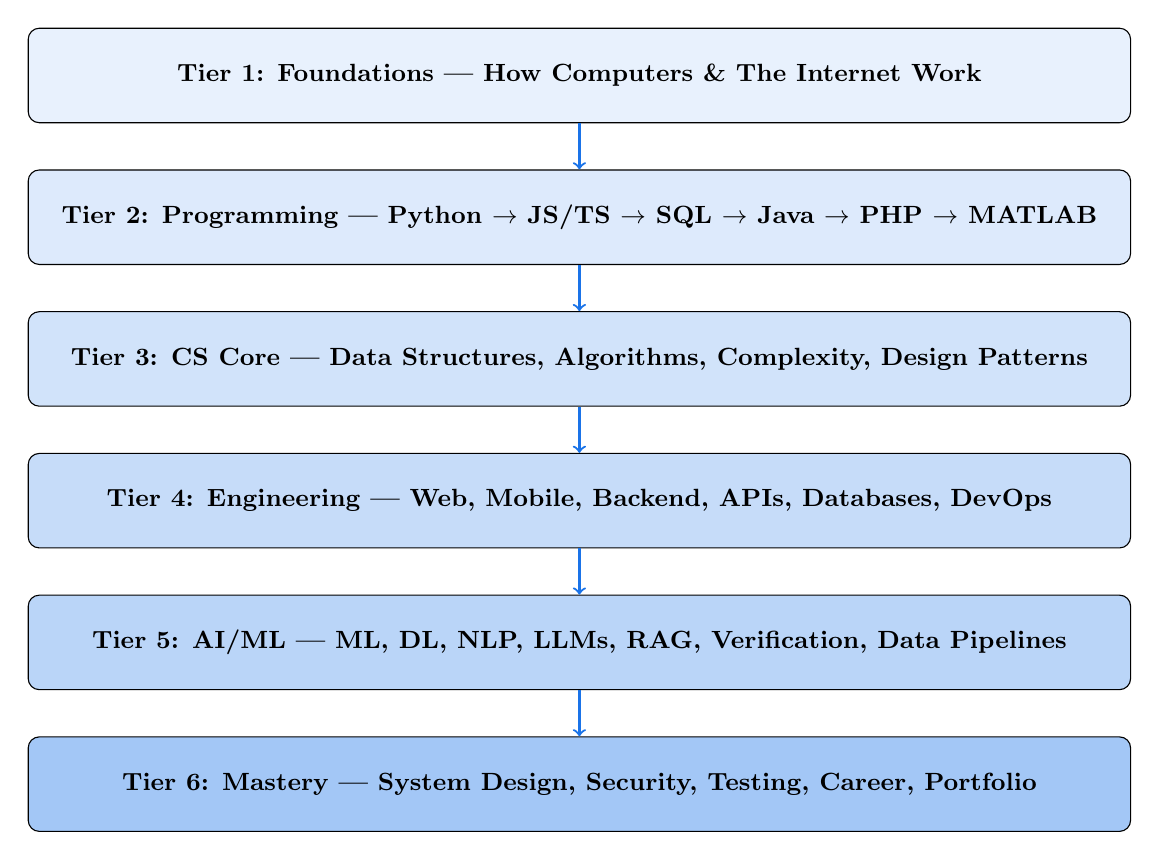
\begin{tikzpicture}[
    tier/.style={draw, rounded corners, minimum width=14cm, minimum height=1.2cm, 
                 text centered, font=\bfseries\small},
    arrow/.style={->, thick, primaryblue}
]
\node[tier, fill=primaryblue!10] (t1) at (0,0) {Tier 1: Foundations — How Computers \& The Internet Work};
\node[tier, fill=primaryblue!15] (t2) at (0,-1.8) {Tier 2: Programming — Python $\to$ JS/TS $\to$ SQL $\to$ Java $\to$ PHP $\to$ MATLAB};
\node[tier, fill=primaryblue!20] (t3) at (0,-3.6) {Tier 3: CS Core — Data Structures, Algorithms, Complexity, Design Patterns};
\node[tier, fill=primaryblue!25] (t4) at (0,-5.4) {Tier 4: Engineering — Web, Mobile, Backend, APIs, Databases, DevOps};
\node[tier, fill=primaryblue!30] (t5) at (0,-7.2) {Tier 5: AI/ML — ML, DL, NLP, LLMs, RAG, Verification, Data Pipelines};
\node[tier, fill=primaryblue!40] (t6) at (0,-9.0) {Tier 6: Mastery — System Design, Security, Testing, Career, Portfolio};

\draw[arrow] (t1) -- (t2);
\draw[arrow] (t2) -- (t3);
\draw[arrow] (t3) -- (t4);
\draw[arrow] (t4) -- (t5);
\draw[arrow] (t5) -- (t6);
\end{tikzpicture}
\end{center}

\newpage

\section{Detailed Roadmap with Chapters}

\subsection{Tier 1 — Foundations Before Coding (Chapters 2--3)}

\textbf{Goal:} Understand what computers are, how they work, how the internet works, and what programming is before writing a single line of code.

\begin{longtable}{p{0.5\textwidth} p{0.45\textwidth}}
\toprule
\textbf{Topic} & \textbf{Chapter / Section} \\
\midrule
\endhead
How computers work (hardware, CPU, memory, storage) & Ch.\ 2, Sec.\ 2.1 \\
Software vs.\ hardware & Ch.\ 2, Sec.\ 2.2 \\
Operating systems (what they are, what they do) & Ch.\ 2, Sec.\ 2.3 \\
Files, folders, directories, paths & Ch.\ 2, Sec.\ 2.4 \\
Terminals, shells, and command-line basics & Ch.\ 2, Sec.\ 2.5 \\
Text editors and IDEs & Ch.\ 2, Sec.\ 2.6 \\
How the internet works (IP, DNS, HTTP/S, ports) & Ch.\ 2, Sec.\ 2.7 \\
Client--server architecture & Ch.\ 2, Sec.\ 2.8 \\
Request/response lifecycle & Ch.\ 2, Sec.\ 2.9 \\
What programming is & Ch.\ 3, Sec.\ 3.1 \\
How code runs (interpreters vs.\ compilers) & Ch.\ 3, Sec.\ 3.2 \\
Algorithmic thinking, pseudocode, flowcharts & Ch.\ 3, Sec.\ 3.3 \\
Problem decomposition & Ch.\ 3, Sec.\ 3.4 \\
\bottomrule
\end{longtable}

\subsection{Tier 2 — Programming Mastery (Chapters 4--10)}

\textbf{Goal:} Learn to code from scratch, starting with Python, then mastering every language in your stack.

\begin{longtable}{p{0.5\textwidth} p{0.45\textwidth}}
\toprule
\textbf{Topic} & \textbf{Chapter / Section} \\
\midrule
\endhead
Programming fundamentals (variables, types, control flow, functions, OOP) & Ch.\ 4 \\
Python mastery (syntax, libraries, ecosystem, best practices) & Ch.\ 5 \\
JavaScript mastery (ES6+, async, DOM, ecosystem) & Ch.\ 6 \\
TypeScript mastery (types, interfaces, generics, with React) & Ch.\ 7 \\
SQL mastery (queries, joins, subqueries, optimisation) & Ch.\ 8 \\
Java mastery (OOP, JVM, collections, concurrency basics) & Ch.\ 9 \\
PHP mastery (syntax, web use, Laravel awareness) & Ch.\ 10 \\
MATLAB mastery (matrices, plotting, engineering use) & Ch.\ 11 \\
\bottomrule
\end{longtable}

\subsection{Tier 3 — Computer Science Core (Chapter 12)}

\textbf{Goal:} Build the theoretical foundation that separates a coder from a software engineer.

\begin{longtable}{p{0.5\textwidth} p{0.45\textwidth}}
\toprule
\textbf{Topic} & \textbf{Chapter / Section} \\
\midrule
\endhead
Arrays, linked lists, stacks, queues & Ch.\ 12, Sec.\ 12.1--12.4 \\
Hash maps and sets & Ch.\ 12, Sec.\ 12.5 \\
Trees (binary, BST, heaps) & Ch.\ 12, Sec.\ 12.6 \\
Graphs (BFS, DFS, shortest path) & Ch.\ 12, Sec.\ 12.7 \\
Recursion and backtracking & Ch.\ 12, Sec.\ 12.8 \\
Sorting algorithms & Ch.\ 12, Sec.\ 12.9 \\
Searching algorithms & Ch.\ 12, Sec.\ 12.10 \\
Big O, time and space complexity & Ch.\ 12, Sec.\ 12.11 \\
Object-oriented design and design patterns & Ch.\ 12, Sec.\ 12.12 \\
Concurrency basics & Ch.\ 12, Sec.\ 12.13 \\
\bottomrule
\end{longtable}

\subsection{Tier 4 — Full-Stack Engineering (Chapters 13--22)}

\textbf{Goal:} Build production-quality web, mobile, and backend applications with real databases and deployment.

\begin{longtable}{p{0.5\textwidth} p{0.45\textwidth}}
\toprule
\textbf{Topic} & \textbf{Chapter / Section} \\
\midrule
\endhead
HTML, CSS, responsive design, Bootstrap & Ch.\ 13 \\
React and frontend engineering & Ch.\ 14 \\
React Native and Expo (mobile engineering) & Ch.\ 15 \\
Backend fundamentals (servers, REST, JSON, auth) & Ch.\ 16 \\
Django and Django REST Framework & Ch.\ 17 \\
Flask & Ch.\ 18 \\
Node.js and Express & Ch.\ 19 \\
Databases, SQL design, ORMs, indexing & Ch.\ 20 \\
Git and GitHub & Ch.\ 21 \\
Docker, CI/CD, Jenkins & Ch.\ 22 \\
\bottomrule
\end{longtable}

\subsection{Tier 5 — AI, ML \& Data Engineering (Chapters 23--29)}

\textbf{Goal:} Learn data pipelines, machine learning, deep learning, NLP, LLMs, RAG, and verification from first principles.

\begin{longtable}{p{0.5\textwidth} p{0.45\textwidth}}
\toprule
\textbf{Topic} & \textbf{Chapter / Section} \\
\midrule
\endhead
ETL, data pipelines, analytics & Ch.\ 23 \\
Pandas, NumPy, Matplotlib & Ch.\ 24 \\
Power BI and Tableau & Ch.\ 25 \\
Machine learning with Scikit-learn & Ch.\ 26 \\
Deep learning with TensorFlow (CNNs, ResNet) & Ch.\ 27 \\
NLP with spaCy & Ch.\ 28 \\
LLM integration, RAG, and verification systems & Ch.\ 29 \\
\bottomrule
\end{longtable}

\subsection{Tier 6 — Mastery, Design \& Career (Chapters 30--41)}

\textbf{Goal:} Become a complete, production-capable, interview-ready engineer.

\begin{longtable}{p{0.5\textwidth} p{0.45\textwidth}}
\toprule
\textbf{Topic} & \textbf{Chapter / Section} \\
\midrule
\endhead
AWS and Kubernetes basics & Ch.\ 30 \\
Security fundamentals & Ch.\ 31 \\
Testing, debugging, documentation & Ch.\ 32 \\
System design and architecture & Ch.\ 33 \\
Project case studies from your CV & Ch.\ 34 \\
Interview and portfolio preparation & Ch.\ 35 \\
30/60/90/180-Day action plan & Ch.\ 36 \\
Glossary of all terms & Ch.\ 37 \\
Final capstone challenges & Ch.\ 38 \\
Next steps to become elite & Ch.\ 39 \\
\bottomrule
\end{longtable}

\newpage

\section{Time Estimates}

Below are rough time estimates for a dedicated learner studying 4--6 hours per day:

\begin{center}
\begin{tabular}{l l l}
\toprule
\textbf{Tier} & \textbf{Duration} & \textbf{Cumulative} \\
\midrule
Tier 1: Foundations & 1--2 weeks & 2 weeks \\
Tier 2: Programming & 6--10 weeks & 12 weeks \\
Tier 3: CS Core & 4--6 weeks & 18 weeks \\
Tier 4: Full-Stack Engineering & 10--14 weeks & 32 weeks \\
Tier 5: AI/ML/Data & 8--12 weeks & 44 weeks \\
Tier 6: Mastery \& Career & 4--6 weeks & 50 weeks \\
\bottomrule
\end{tabular}
\end{center}

\begin{notebox}
These are estimates for deep learning with exercises and projects. If you already have some knowledge (which you do from your degree), certain sections will go faster. However, \textbf{do not skip sections}---use the time to reinforce and fill gaps.
\end{notebox}

\section{How Your CV Projects Map to the Curriculum}

Every project on your CV will be used as a case study. Here is where each project connects:

\begin{longtable}{p{0.3\textwidth} p{0.65\textwidth}}
\toprule
\textbf{Project} & \textbf{Relevant Chapters} \\
\midrule
\endhead
RevSync & Django, DRF, React Native, REST APIs, Docker, System Design, Security, Mobile Engineering \\
VeriRAG & NLP, LLMs, RAG, Verification, Python, Data Pipelines, spaCy, Evaluation \\
AgriXnest & ML, Image Classification, TensorFlow, Backend, API Design \\
CareerForge AI & LLM Integration, NLP, Resume Parsing, Django, Frontend \\
Breast Cancer Detection & Deep Learning, CNNs, ResNet, TensorFlow, Evaluation Metrics \\
Live Chat Bot & Flask, WebSockets (Socket.IO), Real-time Systems \\
MyMusic Maestro & Django, Templates, CRUD, Database Design \\
Giving GRACE & Full-Stack, Event Matching, Django, Frontend \\
\bottomrule
\end{longtable}

\checkpoint{Before proceeding to Chapter 2, make sure you understand the roadmap structure and have set up your study schedule. You know what is ahead. Now let us begin.}


% ============================================================
% CHAPTER 2 — FOUNDATIONS BEFORE CODING
% ============================================================
\chapter{Foundations Before Coding}

Before you write a single line of code, you must understand \textbf{what a computer is}, \textbf{how it works}, \textbf{how the internet works}, and \textbf{what programming actually means}. This chapter assumes you know absolutely nothing.

\section{How Computers Work}

\subsection{What Is a Computer?}

A computer is a machine that takes \textbf{input}, \textbf{processes} it according to a set of \textbf{instructions}, and produces \textbf{output}.

\textbf{Analogy:} Think of a computer like a very obedient, very fast, but very literal employee. It will do exactly what you tell it, extremely quickly, but it cannot think for itself. If you give it bad instructions, it will produce bad results---without complaint.

The key components of any computer are:

\begin{itemize}[leftmargin=2em]
    \item \textbf{CPU (Central Processing Unit):} The ``brain'' of the computer. It executes instructions one at a time (or in parallel on modern processors), performing calculations and making decisions.
    \item \textbf{RAM (Random Access Memory):} Short-term memory. When a program runs, its data and instructions are loaded into RAM because RAM is extremely fast. However, RAM is \textbf{volatile}---when you turn off the computer, everything in RAM is lost.
    \item \textbf{Storage (Hard Drive / SSD):} Long-term memory. Files, programs, photos, documents---everything you want to keep permanently is stored here. Storage is slower than RAM but \textbf{persistent}---it survives power-offs.
    \item \textbf{Motherboard:} The main circuit board that connects all components together. Think of it as the nervous system of the computer.
    \item \textbf{Input devices:} Keyboard, mouse, microphone, camera---anything that sends data \emph{into} the computer.
    \item \textbf{Output devices:} Monitor, speakers, printer---anything that presents data \emph{from} the computer to you.
\end{itemize}

\subsection{Binary: The Language of Computers}

Computers do not understand English, Python, or JavaScript. At the lowest level, they understand only \textbf{binary}: sequences of \textbf{0s and 1s}.

\begin{itemize}[leftmargin=2em]
    \item A single 0 or 1 is called a \textbf{bit} (binary digit).
    \item 8 bits together form a \textbf{byte}.
    \item A byte can represent $2^8 = 256$ different values (0 to 255).
\end{itemize}

\textbf{Why binary?} Because computer hardware is made of tiny electronic switches (transistors) that can be either \textbf{on} (1) or \textbf{off} (0). Everything---numbers, letters, images, videos, programs---is ultimately represented as patterns of 0s and 1s.

\textbf{Example:}
\begin{itemize}[leftmargin=2em]
    \item The number 5 in binary is \texttt{00000101}.
    \item The letter `A' in ASCII encoding is \texttt{01000001} (decimal 65).
    \item The colour white in RGB is three bytes: \texttt{11111111 11111111 11111111} (255, 255, 255).
\end{itemize}

\begin{notebox}
You do not need to memorise binary conversions. The important thing is to understand that \textbf{everything} in a computer is ultimately binary, and that higher-level languages (like Python) exist to save you from having to work in binary directly.
\end{notebox}

\subsection{How the CPU Executes Instructions}

The CPU follows a cycle called the \textbf{fetch--decode--execute} cycle:

\begin{enumerate}[leftmargin=2em]
    \item \textbf{Fetch:} The CPU fetches the next instruction from memory (RAM).
    \item \textbf{Decode:} The CPU decodes the instruction to understand what operation to perform.
    \item \textbf{Execute:} The CPU performs the operation (e.g., add two numbers, compare values, move data).
\end{enumerate}

This cycle repeats billions of times per second on a modern processor. A CPU running at 3 GHz performs roughly 3 billion cycles per second.

\textbf{Key concept:} A ``program'' is just a list of these instructions stored in memory. When you ``run'' a program, the CPU starts reading and executing those instructions one by one.

\subsection{How Memory Works}

Memory in a computer can be visualised as a long row of numbered boxes, each capable of holding one byte:

\begin{verbatim}
Address:  [0000] [0001] [0002] [0003] [0004] ...
Value:    [ 42 ] [ 65 ] [ 00 ] [ 13 ] [ 72 ] ...
\end{verbatim}

\begin{itemize}[leftmargin=2em]
    \item Each box has a unique \textbf{address} (a number identifying its position).
    \item Each box holds a \textbf{value} (one byte of data).
    \item When your program says ``store the number 42'', the CPU puts \texttt{42} into a specific memory address.
    \item When your program says ``read that number back'', the CPU looks up that address and retrieves the value.
\end{itemize}

This is why computer scientists talk about ``memory addresses'' and ``pointers''. At the lowest level, every piece of data your program uses has a specific location in memory.

\section{Software vs.\ Hardware}

\subsection{Definitions}

\begin{itemize}[leftmargin=2em]
    \item \textbf{Hardware:} The physical components you can touch---CPU, RAM, hard drive, monitor, keyboard.
    \item \textbf{Software:} The instructions (programs) that tell the hardware what to do. Software is intangible---you cannot touch it.
\end{itemize}

\subsection{Types of Software}

\begin{enumerate}[leftmargin=2em]
    \item \textbf{System software:} The operating system (macOS, Windows, Linux) and utilities that manage the hardware and provide a platform for other software.
    \item \textbf{Application software:} Programs you use directly---web browsers, text editors, games, your Django apps.
    \item \textbf{Firmware:} Software embedded into hardware devices (e.g., the software inside your router, or the ECU firmware in RevSync).
\end{enumerate}

\begin{projectbox}
\textbf{RevSync} involves ECU (Engine Control Unit) tuning. An ECU contains \textbf{firmware}---software burned into a chip inside the motorcycle's engine management system. Your RevSync project reads, modifies, and re-flashes this firmware. Understanding the hardware--software boundary is directly relevant.
\end{projectbox}

\section{Operating Systems}

\subsection{What Is an Operating System?}

An \textbf{operating system (OS)} is the software layer that sits between you (and your applications) and the hardware. It manages:

\begin{itemize}[leftmargin=2em]
    \item \textbf{Processes:} Running programs. The OS decides which programs get CPU time and for how long.
    \item \textbf{Memory:} The OS allocates RAM to programs and reclaims it when they finish.
    \item \textbf{File system:} The OS organises files on your storage device into folders and directories.
    \item \textbf{I/O (Input/Output):} The OS manages communication between programs and devices (keyboard, screen, network, etc.).
    \item \textbf{Security:} The OS controls who can access what (user accounts, permissions, etc.).
\end{itemize}

\subsection{Common Operating Systems}

\begin{itemize}[leftmargin=2em]
    \item \textbf{macOS:} Used on Apple computers. Based on Unix. You are using this.
    \item \textbf{Windows:} Most common desktop OS worldwide. Used heavily in enterprise.
    \item \textbf{Linux:} Open-source OS. Dominates servers, cloud infrastructure, and DevOps. Essential to learn.
    \item \textbf{Android:} Mobile OS based on Linux. Relevant for mobile development.
    \item \textbf{iOS:} Apple's mobile OS. React Native lets you target both iOS and Android.
\end{itemize}

\begin{tipbox}
As a software engineer, you should be comfortable on macOS and Linux at minimum. Most servers in the world run Linux, and most development tools are designed for Unix-like systems.
\end{tipbox}

\section{Files, Folders, Directories, and Paths}

\subsection{The File System}

Every operating system organises data using a \textbf{file system}: a hierarchical (tree-like) structure of \textbf{files} and \textbf{directories} (folders).

\begin{verbatim}
/
├── Users/
│   └── ayooluwakarim/
│       ├── Documents/
│       │   └── report.pdf
│       ├── Desktop/
│       ├── RevSync-Mac/
│       │   ├── backend/
│       │   ├── mobile/
│       │   └── README.md
│       └── .zshrc
├── Applications/
├── System/
└── tmp/
\end{verbatim}

\subsection{Key Concepts}

\begin{itemize}[leftmargin=2em]
    \item \textbf{Root directory:} The top of the file system tree. On macOS/Linux, it is \texttt{/}. On Windows, it is \texttt{C:\textbackslash}.
    \item \textbf{Home directory:} Your personal directory. On macOS, it is \texttt{/Users/ayooluwakarim}. Abbreviated as \texttt{\textasciitilde}.
    \item \textbf{Absolute path:} The full path from the root. Example: \texttt{/Users/ayooluwakarim/RevSync-Mac/README.md}.
    \item \textbf{Relative path:} A path relative to your current location. If you are in \texttt{RevSync-Mac}, then \texttt{./README.md} refers to the README file.
    \item \textbf{Hidden files:} Files starting with a dot (\texttt{.}) are hidden by default. Example: \texttt{.zshrc}, \texttt{.gitignore}.
\end{itemize}

\begin{warningbox}
Path separators differ between operating systems: macOS/Linux use \texttt{/} (forward slash), Windows uses \texttt{\textbackslash} (backslash). This is a common source of bugs in cross-platform code.
\end{warningbox}

\section{Terminals, Shells, and Command-Line Basics}

\subsection{What Is a Terminal?}

A \textbf{terminal} (also called a \textbf{command line} or \textbf{console}) is a text-based interface to your computer. Instead of clicking buttons and icons, you \textbf{type commands}.

\textbf{Why use a terminal?} Because it is:
\begin{itemize}[leftmargin=2em]
    \item \textbf{Faster} for many tasks (creating files, navigating directories, running programs).
    \item \textbf{More powerful}---you can chain commands, write scripts, automate tasks.
    \item \textbf{Essential} for software development, DevOps, and server management.
    \item \textbf{Universal}---every server you will ever work with has a command line, but may not have a graphical interface.
\end{itemize}

\subsection{What Is a Shell?}

The \textbf{shell} is the program that interprets the commands you type. Common shells:

\begin{itemize}[leftmargin=2em]
    \item \textbf{zsh} (Z shell): Default on modern macOS. You are using this.
    \item \textbf{bash} (Bourne Again Shell): Default on most Linux systems. Very similar to zsh.
    \item \textbf{sh} (Bourne shell): The original Unix shell.
    \item \textbf{PowerShell}: Windows command-line shell.
\end{itemize}

\subsection{Essential Commands}

Here are the commands you must know from day one:

\begin{lstlisting}[language=bash, caption={Essential terminal commands}]
# Navigation
pwd                 # Print working directory (where am I?)
ls                  # List files in current directory
ls -la              # List ALL files (including hidden), with details
cd foldername       # Change directory into 'foldername'
cd ..               # Go up one directory
cd ~                # Go to home directory

# File operations
touch filename.txt  # Create an empty file
mkdir foldername    # Create a new directory
cp source dest      # Copy a file
mv source dest      # Move (or rename) a file
rm filename.txt     # Delete a file (CAREFUL: no recycle bin!)
rm -r foldername    # Delete a directory and everything inside it

# Viewing files
cat filename.txt    # Print entire file contents
head filename.txt   # Print first 10 lines
tail filename.txt   # Print last 10 lines
less filename.txt   # View file with scrolling (press q to quit)

# Searching
grep "text" file    # Search for "text" in a file
find . -name "*.py" # Find all .py files in current directory tree

# System info
whoami              # Print your username
man command         # Show manual page for a command
clear               # Clear the terminal screen
history             # Show command history

# Permissions
chmod +x script.sh  # Make a file executable
\end{lstlisting}

\begin{exercisebox}
\textbf{Exercise 2.1:} Open your terminal (on macOS, open the Terminal app or iTerm2). Try every command listed above. Create a folder called \texttt{bootcamp-practice}, navigate into it, create a file called \texttt{hello.txt}, write something into it using \texttt{echo "Hello World" > hello.txt}, then view its contents with \texttt{cat}.
\end{exercisebox}

\section{Text Editors and IDEs}

\subsection{What Is a Text Editor?}

A \textbf{text editor} is a program for writing and editing plain text files---including code. Unlike a word processor (like Microsoft Word), a text editor does \textbf{not} add formatting (bold, italics, etc.). Code must be plain text.

\subsection{What Is an IDE?}

An \textbf{IDE (Integrated Development Environment)} is a text editor with extra features built in:

\begin{itemize}[leftmargin=2em]
    \item \textbf{Syntax highlighting:} Colours different parts of your code (keywords, strings, comments) to make it readable.
    \item \textbf{Auto-completion:} Suggests code as you type.
    \item \textbf{Debugging tools:} Let you step through your code line by line to find bugs.
    \item \textbf{Integrated terminal:} A command line built into the editor.
    \item \textbf{Version control integration:} Git support built in.
    \item \textbf{Extensions/plugins:} Add support for different languages, tools, and frameworks.
\end{itemize}

\subsection{Recommended: Visual Studio Code (VS Code)}

For this handbook, the recommended editor is \textbf{Visual Studio Code (VS Code)}:
\begin{itemize}[leftmargin=2em]
    \item Free and open source.
    \item Works on macOS, Windows, and Linux.
    \item Enormous extension ecosystem.
    \item Excellent support for Python, JavaScript, TypeScript, and every language in your stack.
    \item Built-in terminal, Git support, and debugger.
\end{itemize}

\begin{tipbox}
Install these VS Code extensions to start: \textbf{Python}, \textbf{Pylance}, \textbf{ESLint}, \textbf{Prettier}, \textbf{GitLens}, \textbf{Docker}, and \textbf{Thunder Client} (for API testing).
\end{tipbox}

\section{How the Internet Works}

\subsection{The Big Picture}

The internet is a \textbf{global network of computers} that can communicate with each other using agreed-upon rules called \textbf{protocols}.

When you type \texttt{https://www.google.com} into your browser, a complex chain of events happens in milliseconds:

\begin{enumerate}[leftmargin=2em]
    \item Your browser asks: ``What is the IP address of \texttt{www.google.com}?''
    \item A \textbf{DNS server} responds: ``It is \texttt{142.250.180.4}.''
    \item Your browser opens a connection to that IP address on \textbf{port 443} (HTTPS).
    \item Your browser sends an \textbf{HTTP request}: ``GET me the homepage.''
    \item Google's server receives the request, processes it, and sends back an \textbf{HTTP response} containing HTML, CSS, and JavaScript.
    \item Your browser renders that HTML/CSS/JS into the visual page you see.
\end{enumerate}

Let us break down each component.

\subsection{IP Addresses}

Every device connected to the internet has a unique \textbf{IP (Internet Protocol) address}---a numerical label that identifies it on the network.

\begin{itemize}[leftmargin=2em]
    \item \textbf{IPv4:} Four numbers separated by dots. Example: \texttt{192.168.1.1}. Each number is 0--255. This gives $\sim$4.3 billion possible addresses.
    \item \textbf{IPv6:} Longer format to accommodate more devices. Example: \texttt{2001:0db8:85a3:0000:0000:8a2e:0370:7334}.
    \item \textbf{Localhost:} \texttt{127.0.0.1} always refers to \emph{your own computer}. When you run a local server, you access it at \texttt{http://127.0.0.1} or \texttt{http://localhost}.
\end{itemize}

\subsection{DNS (Domain Name System)}

Humans are bad at remembering numbers. DNS is the ``phone book'' of the internet---it translates human-friendly domain names into IP addresses.

\begin{verbatim}
www.google.com  -->  DNS  -->  142.250.180.4
github.com      -->  DNS  -->  140.82.121.3
\end{verbatim}

\subsection{Ports}

A single server can run many services. \textbf{Ports} are numbered endpoints (0--65535) that differentiate between services on the same machine.

\begin{itemize}[leftmargin=2em]
    \item Port \textbf{80}: HTTP (unencrypted web traffic).
    \item Port \textbf{443}: HTTPS (encrypted web traffic).
    \item Port \textbf{22}: SSH (secure shell---remote server access).
    \item Port \textbf{5432}: PostgreSQL database.
    \item Port \textbf{3000}: Common for Node.js dev servers.
    \item Port \textbf{8000}: Common for Django dev servers.
    \item Port \textbf{8080}: Common alternative HTTP port.
\end{itemize}

When you run your Django server and it says ``Running on \texttt{http://127.0.0.1:8000}'', it means: ``Access me on \emph{this computer}, on port 8000.''

\subsection{HTTP and HTTPS}

\textbf{HTTP (HyperText Transfer Protocol)} is the protocol browsers use to communicate with web servers. It defines how requests and responses are formatted.

\textbf{HTTPS} is HTTP with encryption (TLS/SSL). All modern websites should use HTTPS.

An HTTP request has:
\begin{itemize}[leftmargin=2em]
    \item \textbf{Method:} What action to take. Common methods:
    \begin{itemize}
        \item \texttt{GET} — Retrieve data (``show me the page'').
        \item \texttt{POST} — Send data (``submit this form'').
        \item \texttt{PUT} — Update data (``replace this resource'').
        \item \texttt{PATCH} — Partially update data.
        \item \texttt{DELETE} — Delete data.
    \end{itemize}
    \item \textbf{URL:} Where to send the request. Example: \texttt{/api/users/42/}.
    \item \textbf{Headers:} Metadata about the request (content type, authentication tokens, etc.).
    \item \textbf{Body:} Data sent with the request (for POST/PUT/PATCH). Often in JSON format.
\end{itemize}

An HTTP response has:
\begin{itemize}[leftmargin=2em]
    \item \textbf{Status code:} A number indicating the result:
    \begin{itemize}
        \item \texttt{200} — OK (success).
        \item \texttt{201} — Created (resource was created).
        \item \texttt{301} — Moved Permanently (redirect).
        \item \texttt{400} — Bad Request (client error).
        \item \texttt{401} — Unauthorised (not logged in).
        \item \texttt{403} — Forbidden (no permission).
        \item \texttt{404} — Not Found.
        \item \texttt{500} — Internal Server Error (server broke).
    \end{itemize}
    \item \textbf{Headers:} Metadata about the response.
    \item \textbf{Body:} The actual content (HTML page, JSON data, image, etc.).
\end{itemize}

\begin{interviewbox}
HTTP methods, status codes, and the request/response lifecycle are \textbf{extremely} common in backend and API interviews. You should be able to explain every status code listed above from memory and give a scenario for each.
\end{interviewbox}

\section{Client--Server Architecture}

\subsection{The Model}

Almost all web applications follow a \textbf{client--server} model:

\begin{itemize}[leftmargin=2em]
    \item \textbf{Client:} The program that makes requests. Usually a web browser or a mobile app.
    \item \textbf{Server:} The program that receives requests, processes them, and sends back responses. Your Django or Express app is a server.
\end{itemize}

\begin{verbatim}
[Client (Browser/App)]  -- HTTP Request -->  [Server (Django/Express)]
                                                    |
                                              [Database]
                                                    |
[Client (Browser/App)]  <-- HTTP Response --  [Server (Django/Express)]
\end{verbatim}

\subsection{Frontend vs.\ Backend}

\begin{itemize}[leftmargin=2em]
    \item \textbf{Frontend:} The code that runs on the \emph{client side} (in the browser or on the user's phone). This is what the user sees and interacts with. Technologies: HTML, CSS, JavaScript, React, React Native.
    \item \textbf{Backend:} The code that runs on the \emph{server side}. This handles business logic, database operations, authentication, and API responses. Technologies: Django, Flask, Node.js/Express.
    \item \textbf{Full-stack:} Working on both frontend and backend. This is what your CV describes.
\end{itemize}

\begin{projectbox}
\textbf{RevSync} is a textbook example of client--server architecture. The React Native mobile app is the \textbf{client}. The Django backend is the \textbf{server}. They communicate via REST APIs over HTTP/HTTPS. Understanding this architecture is foundational to understanding your own project.
\end{projectbox}

\section{The Request/Response Lifecycle}

Let us trace exactly what happens when a user opens your RevSync app and loads their profile:

\begin{enumerate}[leftmargin=2em]
    \item User opens the app and navigates to ``Profile''.
    \item The React Native app constructs an HTTP request: \texttt{GET /api/users/me/} with an \texttt{Authorization: Bearer <JWT\_token>} header.
    \item The request travels over the internet (or local network) to your Django server.
    \item Django's URL router matches \texttt{/api/users/me/} to a view function.
    \item The view function checks the JWT token to verify the user is authenticated.
    \item The view function queries the PostgreSQL database for the user's profile data.
    \item The database returns the data (name, email, bike info, etc.).
    \item Django serialises the data into JSON format.
    \item Django sends back an HTTP response with status \texttt{200 OK} and the JSON body.
    \item The React Native app receives the response, parses the JSON, and renders the profile screen.
\end{enumerate}

Every interaction between the app and server follows this pattern. The rest of this handbook will teach you how to build every component in this chain.

\checkpoint{You now understand how computers work, what binary is, what operating systems do, how the file system is organised, how to use a terminal, what the internet is, how HTTP works, and the client--server model. These are the foundations everything else builds on.}


% ============================================================
% CHAPTER 3 — WHAT PROGRAMMING IS
% ============================================================
\chapter{What Programming Is}

\section{Definition}
\textbf{Programming} is the process of writing instructions that a computer can execute to perform a specific task. These instructions are written in a \textbf{programming language}---a formal language with strict syntax rules that can be translated into machine code the CPU understands.

\textbf{Analogy:} Programming is like writing a recipe. The recipe (program) contains step-by-step instructions. The chef (CPU) follows those instructions exactly. If you write ``add salt'' but mean ``add sugar'', the chef will add salt---computers do exactly what you say, not what you mean.

\section{How Code Runs: Interpreters vs.\ Compilers}

Programming languages are designed for humans to read and write, but computers only understand binary machine code. Something must translate your human-readable code into machine code. There are two main approaches:

\subsection{Compiled Languages}
A \textbf{compiler} translates your \emph{entire} source code into machine code \emph{before} the program runs. The output is an executable file that the CPU can run directly.

\begin{itemize}[leftmargin=2em]
    \item \textbf{Examples:} C, C++, Java (partially), Go, Rust.
    \item \textbf{Advantage:} Fast execution---the translation is done once, ahead of time.
    \item \textbf{Disadvantage:} Slower development cycle---you must compile before every run.
\end{itemize}

\subsection{Interpreted Languages}
An \textbf{interpreter} translates your code \emph{line by line} as the program runs. There is no separate compilation step.

\begin{itemize}[leftmargin=2em]
    \item \textbf{Examples:} Python, JavaScript, PHP, Ruby.
    \item \textbf{Advantage:} Fast development---write and run immediately.
    \item \textbf{Disadvantage:} Slower execution---translation happens at runtime.
\end{itemize}

\begin{notebox}
Some languages use a hybrid approach. Java compiles to \textbf{bytecode} (an intermediate form), which is then interpreted by the \textbf{JVM (Java Virtual Machine)}. Python also compiles to bytecode (\texttt{.pyc} files) behind the scenes, but this is transparent to you.
\end{notebox}

\section{Algorithmic Thinking}
Before writing code, you must think about \textbf{how to solve the problem}. This is called \textbf{algorithmic thinking}: breaking a problem into a clear sequence of steps.

\subsection{Pseudocode}
\textbf{Pseudocode} is a way to describe an algorithm in plain English (or structured English) without worrying about programming language syntax.

\begin{lstlisting}[caption={Pseudocode example: finding the largest number in a list}]
ALGORITHM FindLargest(list):
    SET largest = first element of list
    FOR each element in list:
        IF element > largest:
            SET largest = element
    RETURN largest
\end{lstlisting}

\subsection{Problem Decomposition}
Every complex problem can be broken into smaller, manageable sub-problems. This is the single most important skill in programming.

\textbf{Example:} Building a user login system can be decomposed into:
\begin{enumerate}[leftmargin=2em]
    \item Display a login form (frontend)
    \item Capture username and password input
    \item Send credentials to the server (API call)
    \item Validate credentials against the database (backend)
    \item Generate a session token or JWT
    \item Return success/failure response
    \item Store token on the client and redirect
\end{enumerate}

\begin{exercisebox}
\textbf{Exercise 3.1:} Write pseudocode for the following problems: (a) Making a cup of tea. (b) Checking if a number is even or odd. (c) Counting how many vowels are in a word. (d) Finding the average of a list of numbers.
\end{exercisebox}

\checkpoint{You now understand what programming is, how code is translated into machine instructions, what pseudocode is, and how to decompose problems. You are ready to start writing actual code.}


% ============================================================
% CHAPTER 4 — PROGRAMMING FUNDAMENTALS WITH PYTHON
% ============================================================
\chapter{Programming Fundamentals with Python}

We begin coding with \textbf{Python} because it has the cleanest syntax and is used across your entire stack (Django, Flask, ML, data pipelines, VeriRAG, CareerForge AI, etc.).

\section{Setting Up Python}

\begin{lstlisting}[language=bash, caption={Installing and verifying Python}]
# Check if Python is installed
python3 --version

# If not installed (macOS):
brew install python3

# Create a project folder
mkdir ~/bootcamp-python && cd ~/bootcamp-python

# Create a virtual environment
python3 -m venv venv
source venv/bin/activate  # activates the environment

# Verify
which python  # should point to your venv
\end{lstlisting}

\begin{warningbox}
Always use \textbf{virtual environments} for Python projects. A virtual environment isolates your project's packages from the system Python, preventing version conflicts. Every project in your career should have its own virtual environment.
\end{warningbox}

\section{Variables and Data Types}

A \textbf{variable} is a named container that stores a value in memory.

\begin{lstlisting}[language=Python, caption={Variables and basic data types}]
# Integers (whole numbers)
age = 24
year = 2026

# Floats (decimal numbers)
price = 19.99
pi = 3.14159

# Strings (text)
name = "Amzat Karim"
greeting = 'Hello, World!'

# Booleans (True or False)
is_student = True
has_graduated = False

# None (absence of value)
result = None

# Check type
print(type(age))       # <class 'int'>
print(type(price))     # <class 'float'>
print(type(name))      # <class 'str'>
print(type(is_student))# <class 'bool'>
\end{lstlisting}

\subsection{Type Conversion}
\begin{lstlisting}[language=Python, caption={Type conversion}]
# String to int
num_str = "42"
num_int = int(num_str)    # 42

# Int to string
age = 24
age_str = str(age)        # "24"

# Float to int (truncates, does NOT round)
pi = 3.7
pi_int = int(pi)          # 3

# String to float
price_str = "19.99"
price = float(price_str)  # 19.99
\end{lstlisting}

\section{Operators}

\begin{lstlisting}[language=Python, caption={Python operators}]
# Arithmetic
a + b    # Addition
a - b    # Subtraction
a * b    # Multiplication
a / b    # Division (always returns float)
a // b   # Floor division (rounds down to int)
a % b    # Modulo (remainder)
a ** b   # Exponentiation (a to the power of b)

# Comparison (return True/False)
a == b   # Equal
a != b   # Not equal
a > b    # Greater than
a < b    # Less than
a >= b   # Greater than or equal
a <= b   # Less than or equal

# Logical
x and y  # True if BOTH are True
x or y   # True if EITHER is True
not x    # Inverts True/False

# Assignment shortcuts
x += 5   # same as x = x + 5
x -= 3   # same as x = x - 3
x *= 2   # same as x = x * 2
\end{lstlisting}

\section{Conditionals (if/elif/else)}

\begin{lstlisting}[language=Python, caption={Conditional statements}]
age = 24

if age < 13:
    print("Child")
elif age < 18:
    print("Teenager")
elif age < 65:
    print("Adult")
else:
    print("Senior")
# Output: Adult

# Ternary (inline) conditional
status = "adult" if age >= 18 else "minor"
\end{lstlisting}

\begin{warningbox}
Python uses \textbf{indentation} (whitespace) to define code blocks, not curly braces like Java or JavaScript. Incorrect indentation causes \texttt{IndentationError}. Always use 4 spaces per indent level.
\end{warningbox}

\section{Loops}

\begin{lstlisting}[language=Python, caption={Loops in Python}]
# For loop - iterate over a sequence
fruits = ["apple", "banana", "cherry"]
for fruit in fruits:
    print(fruit)

# For loop with range
for i in range(5):        # 0, 1, 2, 3, 4
    print(i)

for i in range(2, 8):     # 2, 3, 4, 5, 6, 7
    print(i)

for i in range(0, 10, 2): # 0, 2, 4, 6, 8
    print(i)

# While loop
count = 0
while count < 5:
    print(count)
    count += 1

# break and continue
for i in range(10):
    if i == 3:
        continue  # skip 3
    if i == 7:
        break     # stop at 7
    print(i)      # prints 0, 1, 2, 4, 5, 6

# enumerate (get index AND value)
for index, fruit in enumerate(fruits):
    print(f"{index}: {fruit}")
\end{lstlisting}

\section{Functions}

\begin{lstlisting}[language=Python, caption={Functions}]
# Basic function
def greet(name):
    return f"Hello, {name}!"

message = greet("Amzat")
print(message)  # Hello, Amzat!

# Default parameters
def greet(name, greeting="Hello"):
    return f"{greeting}, {name}!"

# Multiple return values
def divide(a, b):
    quotient = a // b
    remainder = a % b
    return quotient, remainder

q, r = divide(17, 5)  # q=3, r=2

# *args and **kwargs
def flexible(*args, **kwargs):
    print(f"Positional: {args}")
    print(f"Keyword: {kwargs}")

flexible(1, 2, 3, name="Amzat", age=24)
# Positional: (1, 2, 3)
# Keyword: {'name': 'Amzat', 'age': 24}
\end{lstlisting}

\section{Data Structures}

\subsection{Lists}
\begin{lstlisting}[language=Python, caption={Lists}]
# Ordered, mutable, allows duplicates
numbers = [1, 2, 3, 4, 5]
mixed = [1, "hello", True, 3.14]

# Access
numbers[0]    # 1 (first element)
numbers[-1]   # 5 (last element)
numbers[1:3]  # [2, 3] (slicing)

# Modify
numbers.append(6)       # Add to end
numbers.insert(0, 0)    # Insert at index
numbers.remove(3)       # Remove first occurrence of 3
popped = numbers.pop()  # Remove and return last
numbers.sort()          # Sort in place
numbers.reverse()       # Reverse in place

# List comprehension
squares = [x**2 for x in range(10)]
evens = [x for x in range(20) if x % 2 == 0]
\end{lstlisting}

\subsection{Dictionaries}
\begin{lstlisting}[language=Python, caption={Dictionaries}]
# Key-value pairs, unordered (insertion-ordered in 3.7+)
user = {
    "name": "Amzat Karim",
    "age": 24,
    "city": "London",
    "skills": ["Python", "Django", "React Native"]
}

# Access
user["name"]           # "Amzat Karim"
user.get("email", "N/A")  # "N/A" (safe access with default)

# Modify
user["email"] = "karimamzat26@gmail.com"
del user["age"]

# Iteration
for key, value in user.items():
    print(f"{key}: {value}")

# Dictionary comprehension
squares = {x: x**2 for x in range(5)}
\end{lstlisting}

\subsection{Tuples and Sets}
\begin{lstlisting}[language=Python, caption={Tuples and Sets}]
# Tuples: ordered, IMMUTABLE
coordinates = (51.5074, -0.1278)  # London
x, y = coordinates  # unpacking

# Sets: unordered, unique elements, no duplicates
unique_nums = {1, 2, 3, 3, 4}  # {1, 2, 3, 4}
a = {1, 2, 3}
b = {2, 3, 4}
a | b   # Union: {1, 2, 3, 4}
a & b   # Intersection: {2, 3}
a - b   # Difference: {1}
\end{lstlisting}

\section{String Operations}

\begin{lstlisting}[language=Python, caption={String methods}]
name = "Amzat Karim"
name.upper()         # "AMZAT KARIM"
name.lower()         # "amzat karim"
name.split(" ")      # ["Amzat", "Karim"]
name.replace("Karim", "K")  # "Amzat K"
name.startswith("Am")       # True
name.strip()         # Remove whitespace from both ends
" ".join(["a", "b"]) # "a b"

# f-strings (formatted strings) - Python 3.6+
age = 24
print(f"I am {age} years old")
print(f"Next year I'll be {age + 1}")
print(f"Pi is approximately {3.14159:.2f}")  # 3.14
\end{lstlisting}

\section{File Handling}

\begin{lstlisting}[language=Python, caption={File I/O}]
# Writing to a file
with open("output.txt", "w") as f:
    f.write("Hello, World!\n")
    f.write("Second line\n")

# Reading a file
with open("output.txt", "r") as f:
    content = f.read()       # entire file as string

with open("output.txt", "r") as f:
    lines = f.readlines()    # list of lines

# Appending
with open("output.txt", "a") as f:
    f.write("Appended line\n")

# Reading JSON
import json
with open("data.json", "r") as f:
    data = json.load(f)

# Writing JSON
with open("data.json", "w") as f:
    json.dump({"name": "Amzat"}, f, indent=2)
\end{lstlisting}

\begin{tipbox}
Always use the \texttt{with} statement for file operations. It automatically closes the file when the block ends, even if an error occurs. This prevents resource leaks.
\end{tipbox}

\section{Exception Handling}

\begin{lstlisting}[language=Python, caption={Exception handling}]
try:
    result = 10 / 0
except ZeroDivisionError:
    print("Cannot divide by zero!")
except (TypeError, ValueError) as e:
    print(f"Error: {e}")
except Exception as e:
    print(f"Unexpected error: {e}")
else:
    print("No error occurred")  # runs if no exception
finally:
    print("Always runs")  # cleanup code

# Raising exceptions
def withdraw(amount, balance):
    if amount > balance:
        raise ValueError(f"Insufficient funds: {balance}")
    return balance - amount

# Custom exceptions
class InsufficientFundsError(Exception):
    def __init__(self, balance, amount):
        self.balance = balance
        self.amount = amount
        super().__init__(
            f"Cannot withdraw {amount}. Balance: {balance}"
        )
\end{lstlisting}

\section{Object-Oriented Programming (OOP)}

\begin{lstlisting}[language=Python, caption={OOP in Python}]
class Vehicle:
    """Base class for all vehicles."""
    
    def __init__(self, make, model, year):
        self.make = make        # public attribute
        self.model = model
        self.year = year
        self._mileage = 0       # protected (convention)
        self.__vin = None       # private (name mangling)
    
    def drive(self, km):
        self._mileage += km
        return f"Drove {km}km. Total: {self._mileage}km"
    
    def __str__(self):
        return f"{self.year} {self.make} {self.model}"
    
    def __repr__(self):
        return f"Vehicle('{self.make}', '{self.model}', {self.year})"

# Inheritance
class Motorcycle(Vehicle):
    def __init__(self, make, model, year, engine_cc):
        super().__init__(make, model, year)
        self.engine_cc = engine_cc
    
    def wheelie(self):
        return "Doing a wheelie!"

# Usage
bike = Motorcycle("Yamaha", "MT-07", 2024, 689)
print(bike)           # 2024 Yamaha MT-07
print(bike.drive(50)) # Drove 50km. Total: 50km
print(bike.wheelie()) # Doing a wheelie!

# isinstance check
print(isinstance(bike, Vehicle))     # True
print(isinstance(bike, Motorcycle))  # True
\end{lstlisting}

\subsection{Key OOP Concepts}
\begin{itemize}[leftmargin=2em]
    \item \textbf{Encapsulation:} Bundling data and methods together; hiding internal state.
    \item \textbf{Inheritance:} Creating new classes from existing ones (code reuse).
    \item \textbf{Polymorphism:} Different classes responding to the same method call differently.
    \item \textbf{Abstraction:} Hiding complex implementation behind a simple interface.
\end{itemize}

\begin{interviewbox}
OOP is asked in virtually every software engineering interview. Be able to explain the four pillars, give examples, and discuss when inheritance is appropriate vs.\ composition (``has-a'' vs.\ ``is-a'' relationships).
\end{interviewbox}

\section{Modules and Packages}

\begin{lstlisting}[language=Python, caption={Modules and imports}]
# Import entire module
import math
print(math.sqrt(16))  # 4.0

# Import specific items
from math import pi, sqrt
print(pi)  # 3.14159...

# Import with alias
import numpy as np

# Your own modules: create utils.py
# utils.py
def calculate_tax(amount, rate=0.2):
    return amount * rate

# main.py
from utils import calculate_tax
tax = calculate_tax(100)  # 20.0

# Package structure:
# mypackage/
#   __init__.py
#   module_a.py
#   module_b.py
\end{lstlisting}

\section{Decorators}

\begin{lstlisting}[language=Python, caption={Decorators}]
import time

def timer(func):
    """Decorator that measures execution time."""
    def wrapper(*args, **kwargs):
        start = time.time()
        result = func(*args, **kwargs)
        elapsed = time.time() - start
        print(f"{func.__name__} took {elapsed:.4f}s")
        return result
    return wrapper

@timer
def slow_function():
    time.sleep(1)
    return "Done"

slow_function()  # slow_function took 1.0012s
\end{lstlisting}

\begin{projectbox}
Django uses decorators extensively: \texttt{@login\_required}, \texttt{@api\_view}, \texttt{@permission\_classes}, \texttt{@action}. Understanding how decorators work is essential for your Django/DRF projects like RevSync.
\end{projectbox}

\section{Generators and Iterators}

\begin{lstlisting}[language=Python, caption={Generators}]
# Generator function (uses yield instead of return)
def fibonacci(n):
    a, b = 0, 1
    for _ in range(n):
        yield a
        a, b = b, a + b

# Memory-efficient: generates values one at a time
for num in fibonacci(10):
    print(num)  # 0, 1, 1, 2, 3, 5, 8, 13, 21, 34

# Generator expression
squares = (x**2 for x in range(1000000))  # no memory spike
\end{lstlisting}

\section{Lambda Functions and Functional Tools}

\begin{lstlisting}[language=Python, caption={Lambda and functional programming}]
# Lambda: anonymous, single-expression function
square = lambda x: x ** 2
add = lambda a, b: a + b

# map: apply function to every element
numbers = [1, 2, 3, 4, 5]
squared = list(map(lambda x: x**2, numbers))

# filter: keep elements that pass a test
evens = list(filter(lambda x: x % 2 == 0, numbers))

# sorted with key
users = [{"name": "Zoe", "age": 30}, {"name": "Amy", "age": 25}]
sorted_users = sorted(users, key=lambda u: u["age"])
\end{lstlisting}

\section{Recursion}

\begin{lstlisting}[language=Python, caption={Recursion}]
# Factorial: n! = n * (n-1) * ... * 1
def factorial(n):
    if n <= 1:       # base case
        return 1
    return n * factorial(n - 1)  # recursive case

print(factorial(5))  # 120

# Every recursive function MUST have:
# 1. A BASE CASE that stops recursion
# 2. A RECURSIVE CASE that moves toward the base case
\end{lstlisting}

\checkpoint{You now know Python fundamentals: variables, types, operators, conditionals, loops, functions, data structures, OOP, file handling, exceptions, decorators, generators, and recursion. Practice these until they are second nature.}


% ============================================================
% CHAPTER 5 — PYTHON MASTERY
% ============================================================
\chapter{Python Mastery}

This chapter goes deeper into Python's advanced features, standard library, ecosystem, and production best practices.

\section{Advanced OOP}

\begin{lstlisting}[language=Python, caption={Advanced OOP features}]
# Class methods and static methods
class User:
    _count = 0
    
    def __init__(self, name, email):
        self.name = name
        self.email = email
        User._count += 1
    
    @classmethod
    def get_count(cls):
        return cls._count
    
    @staticmethod
    def validate_email(email):
        return "@" in email and "." in email

# Properties (getters/setters)
class Temperature:
    def __init__(self, celsius):
        self._celsius = celsius
    
    @property
    def celsius(self):
        return self._celsius
    
    @celsius.setter
    def celsius(self, value):
        if value < -273.15:
            raise ValueError("Below absolute zero!")
        self._celsius = value
    
    @property
    def fahrenheit(self):
        return self._celsius * 9/5 + 32

# Abstract base classes
from abc import ABC, abstractmethod

class Shape(ABC):
    @abstractmethod
    def area(self):
        pass
    
    @abstractmethod
    def perimeter(self):
        pass

class Circle(Shape):
    def __init__(self, radius):
        self.radius = radius
    
    def area(self):
        return 3.14159 * self.radius ** 2
    
    def perimeter(self):
        return 2 * 3.14159 * self.radius

# Dataclasses (Python 3.7+)
from dataclasses import dataclass, field
from typing import List

@dataclass
class TuneFile:
    name: str
    engine_cc: int
    version: float = 1.0
    tags: List[str] = field(default_factory=list)
    
    def display_name(self):
        return f"{self.name} v{self.version}"
\end{lstlisting}

\section{Type Hints}

\begin{lstlisting}[language=Python, caption={Type hints}]
from typing import List, Dict, Optional, Tuple, Union

def process_users(
    users: List[Dict[str, str]],
    limit: Optional[int] = None
) -> List[str]:
    names = [u["name"] for u in users]
    if limit:
        return names[:limit]
    return names

def get_user(user_id: int) -> Optional[Dict[str, str]]:
    """Returns user dict or None if not found."""
    ...
\end{lstlisting}

\section{Context Managers}

\begin{lstlisting}[language=Python, caption={Context managers}]
# Custom context manager using class
class DatabaseConnection:
    def __enter__(self):
        self.conn = create_connection()
        return self.conn
    
    def __exit__(self, exc_type, exc_val, exc_tb):
        self.conn.close()

# Using contextlib
from contextlib import contextmanager

@contextmanager
def timer(label):
    import time
    start = time.time()
    yield
    print(f"{label}: {time.time() - start:.4f}s")

with timer("Data processing"):
    # ... do work ...
    pass
\end{lstlisting}

\section{Async/Await}

\begin{lstlisting}[language=Python, caption={Asynchronous Python}]
import asyncio

async def fetch_data(url: str) -> dict:
    print(f"Fetching {url}...")
    await asyncio.sleep(1)  # simulates network delay
    return {"url": url, "status": 200}

async def main():
    # Run concurrently (not in parallel)
    results = await asyncio.gather(
        fetch_data("https://api.example.com/users"),
        fetch_data("https://api.example.com/posts"),
        fetch_data("https://api.example.com/comments"),
    )
    for r in results:
        print(r)

asyncio.run(main())
\end{lstlisting}

\section{Testing in Python}

\begin{lstlisting}[language=Python, caption={Testing with pytest}]
# test_calculator.py
import pytest

def add(a, b):
    return a + b

def divide(a, b):
    if b == 0:
        raise ValueError("Cannot divide by zero")
    return a / b

# Basic tests
def test_add():
    assert add(2, 3) == 5
    assert add(-1, 1) == 0
    assert add(0, 0) == 0

# Testing exceptions
def test_divide_by_zero():
    with pytest.raises(ValueError):
        divide(10, 0)

# Parameterized tests
@pytest.mark.parametrize("a, b, expected", [
    (10, 2, 5.0),
    (7, 3, 2.3333333333333335),
    (0, 5, 0.0),
])
def test_divide(a, b, expected):
    assert divide(a, b) == pytest.approx(expected)

# Fixtures
@pytest.fixture
def sample_users():
    return [
        {"name": "Amzat", "age": 24},
        {"name": "Test", "age": 30},
    ]

def test_user_count(sample_users):
    assert len(sample_users) == 2
\end{lstlisting}

\section{Python Standard Library Highlights}

\begin{itemize}[leftmargin=2em]
    \item \texttt{os} / \texttt{pathlib} --- file system operations
    \item \texttt{sys} --- system-level operations, command-line args
    \item \texttt{json} --- JSON encoding/decoding
    \item \texttt{csv} --- CSV file reading/writing
    \item \texttt{datetime} --- date and time manipulation
    \item \texttt{collections} --- \texttt{defaultdict}, \texttt{Counter}, \texttt{deque}, \texttt{OrderedDict}
    \item \texttt{itertools} --- combinatoric iterators
    \item \texttt{functools} --- \texttt{lru\_cache}, \texttt{partial}, \texttt{reduce}
    \item \texttt{re} --- regular expressions
    \item \texttt{logging} --- structured logging
    \item \texttt{typing} --- type hints
    \item \texttt{unittest} / \texttt{pytest} --- testing frameworks
    \item \texttt{hashlib} --- cryptographic hashing
    \item \texttt{secrets} --- secure random values
    \item \texttt{subprocess} --- running external commands
    \item \texttt{http.server} --- simple HTTP server
    \item \texttt{argparse} --- command-line argument parsing
\end{itemize}

\section{Virtual Environments and Package Management}

\begin{lstlisting}[language=bash, caption={Virtual environment workflow}]
# Create virtual environment
python3 -m venv venv

# Activate
source venv/bin/activate    # macOS/Linux
# venv\Scripts\activate     # Windows

# Install packages
pip install django==4.2 requests numpy

# Freeze dependencies
pip freeze > requirements.txt

# Install from requirements
pip install -r requirements.txt

# Deactivate
deactivate
\end{lstlisting}

\section{Python Best Practices}

\begin{enumerate}[leftmargin=2em]
    \item Follow \textbf{PEP 8} (Python style guide): 4-space indentation, snake\_case for functions/variables, PascalCase for classes.
    \item Write \textbf{docstrings} for every function and class.
    \item Use \textbf{type hints} for all function signatures.
    \item Use \textbf{virtual environments} for every project.
    \item Use \textbf{f-strings} (not \texttt{\%} formatting or \texttt{.format()}).
    \item Handle errors with specific exception types, never bare \texttt{except:}.
    \item Use \texttt{with} for file and resource management.
    \item Write \textbf{tests} (aim for at least 80\% coverage).
    \item Use a linter (\texttt{flake8}) and formatter (\texttt{black}).
    \item Keep functions short (under 20 lines ideally).
\end{enumerate}

\checkpoint{You now have deep Python knowledge covering advanced OOP, type hints, context managers, async, testing, the standard library, and best practices. Python is the foundation for Django, Flask, ML, and data engineering---everything that follows builds on this.}


% ============================================================
% REMAINING CHAPTERS CONTINUE BELOW
% ============================================================
%%INSERTION_POINT_1%%

\end{document}
